\propriete
    [\exmplist
        {27,32 -- 18,1 devient :\\ \opsub[carrysub, lastcarry, deletezero=false]{27.32}{18.1}}{8768--12792 devient :\\ \opsub[carrysub, lastcarry, deletezero=false]{12792}{8768}}{0,0001--11,2 devient :\\ \opsub[carrysub, lastcarry, deletezero=false]{11.2}{0.0001}}]
{Poser une soustraction}
{On va ici poser la soustraction 18,28 - 9,154.\\    
\begin{minipage}{0.7\textwidth}    
On pose les deux nombres à additionner l'un en dessous de l'autre, \textcolor{red}{en alignant les chiffres des unités} (\textcolor{teal}{les virgules seront donc aussi alignées}), et \textcolor{blue}{on complête à gauche et à droite par des 0} pour avoir autant de chiffres.   
\end{minipage}
\hfill
\begin{minipage}{0.22\textwidth}
    \begin{figure}[H]
    \centering
        \resizebox{\textwidth}{!}{
            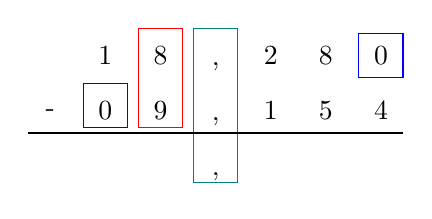
\begin{tikzpicture}[scale=0.7]
                \draw (0,0) node {1} ;
                \draw (1,0) node {8} ; 
                \draw (2,-0.2) node {,} ;
                \draw (3,0) node {2} ;
                \draw (4,0) node {8} ;
                \draw (5,0)  node {0} ;
                \draw  [blue] (-0.4,-0.5) rectangle (0.4,-1.3);
                \draw  [blue] (4.6,0.4) rectangle (5.4,-0.4) ;
                \draw (0,-1) node {0} ;
                \draw (1,-1) node {9} ; 
                \draw (2,-1.2) node {,} ;
                \draw (2,-2.2) node {,} ;
                \draw [teal] (1.6,0.5) rectangle (2.4,-2.3);
                \draw (3,-1) node {1} ;
                \draw (4,-1) node {5} ;
                \draw (5,-1) node {4} ;
                \draw (-1,-1) node {-} ;
                \draw (-1.4,-1.4) -- (5.4,-1.4) ;
                \draw [red] (0.6,0.5) rectangle (1.4,-1.3);
            \end{tikzpicture}
        }
    \end{figure}
\end{minipage}
\\\vspace{1em}\\
\begin{minipage}{0.7\textwidth}    
    On soustrait les nombres par colone, \textcolor{red}{de droite à gauche}. \\
    Si le nombre à soustraire est le plus grand (ici, 4 est plus grand que 0), on met \textcolor{teal}{une retenue}. Le 0 devient un 10 et le prochain nombre à soustraire reçoit un +1
\end{minipage}
\hfill
\begin{minipage}{0.22\textwidth}
    \begin{figure}[H]
    \centering
        \resizebox{\textwidth}{!}{
            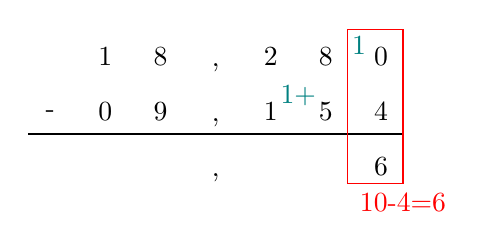
\begin{tikzpicture}[scale=0.7]
                \draw (0,0) node {1} ;
                \draw (1,0) node {8} ; 
                \draw (2,-0.2) node {,} ;
                \draw (3,0) node {2} ;
                \draw (4,0) node {8} ;
                \draw (5,0)  node {0} ;
                \draw [teal] (4.6,0.2)  node {1} ;
                \draw (5,-2)  node {6} ;
                \draw (0,-1) node {0} ;
                \draw (1,-1) node {9} ; 
                \draw (2,-1.2) node {,} ;
                \draw (2,-2.2) node {,} ;
                \draw (3,-1) node {1} ;
                \draw (4,-1) node {5} ;
                \draw [teal] (3.5,-0.7) node {1+} ;
                \draw (5,-1) node {4} ;
                \draw (-1,-1) node {-} ;
                \draw (-1.4,-1.4) -- (5.4,-1.4) ;
                \draw [red] (4.4,0.5) rectangle (5.4,-2.3) node [below] {10-4=6};
            \end{tikzpicture}
        }
    \end{figure}
\end{minipage}
\begin{minipage}{0.7\textwidth}    
    On prend ensuite la colone suivante (vers la gauche) et on recommence,\textcolor{teal}{ sans oublier la retenue}. 
\end{minipage}
\hfill
\begin{minipage}{0.22\textwidth}
    \begin{figure}[H]
    \centering
        \resizebox{\textwidth}{!}{
            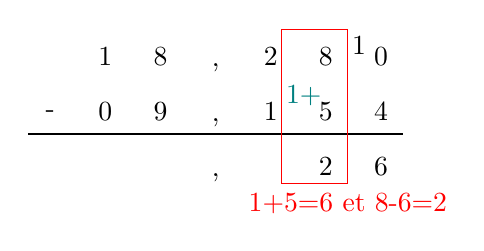
\begin{tikzpicture}[scale=0.7]
                \draw (0,0) node {1} ;
                \draw (1,0) node {8} ; 
                \draw (2,-0.2) node {,} ;
                \draw (3,0) node {2} ;
                \draw (4,0) node {8} ;
                \draw (5,0)  node {0} ;
                \draw (4.6,0.2)  node {1} ;
                \draw (5,-2)  node {6} ;
                \draw (0,-1) node {0} ;
                \draw (1,-1) node {9} ; 
                \draw (2,-1.2) node {,} ;
                \draw (2,-2.2) node {,} ;
                \draw (3,-1) node {1} ;
                \draw (4,-1) node {5} ;
                \draw (4,-2) node {2} ;
                \draw [teal] (3.6,-0.7) node {1+} ;
                \draw (5,-1) node {4} ;
                \draw (-1,-1) node {-} ;
                \draw (-1.4,-1.4) -- (5.4,-1.4) ;
                \draw [red] (3.2,0.5) rectangle (4.4,-2.3) node [below] {1+5=6 et 8-6=2};
            \end{tikzpicture}
        }
    \end{figure}
\end{minipage}
\begin{minipage}{0.7\textwidth}    
    On continue en remontant vers la gauche. On a donc :
    \begin{itemize}
        \item \textcolor{teal}{2-1=1}
        \item \textcolor{red}{On met une retenue. 18-9=9}
        \item \textcolor{blue}{On oublie pas la retenue. 0+1=1 On a donc 1-1=0}
    \end{itemize} 
\end{minipage}
\hfill
\begin{minipage}{0.22\textwidth}
    \begin{figure}[H]
    \centering
        \resizebox{\textwidth}{!}{
            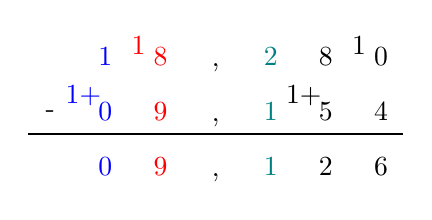
\begin{tikzpicture}[scale=0.7]
                \draw [blue] (0,0) node {1} ;
                \draw [red] (1,0) node {8} ; 
                \draw (2,-0.2) node {,} ;
                \draw [teal] (3,0) node {2} ;
                \draw (4,0) node {8} ;
                \draw (5,0)  node {0} ;
                \draw [red] (0.6,0.2)  node {1} ;
                \draw (4.6,0.2)  node {1} ;
                \draw (5,-2)  node {6} ;
                \draw [blue] (0,-1) node {0} ;
                \draw [blue] (0,-2) node {0} ;
                \draw [red] (1,-1) node {9} ; 
                \draw [red] (1,-2) node {9} ;
                \draw (2,-1.2) node {,} ;
                \draw (2,-2.2) node {,} ;
                \draw [teal] (3,-1) node {1} ;
                \draw (4,-1) node {5} ;
                \draw (4,-2) node {2} ;
                \draw [teal] (3,-2) node {1} ;
                \draw (3.6,-0.7) node {1+} ;
                \draw [blue] (-0.4,-0.7) node {1+} ;
                \draw (5,-1) node {4} ;
                \draw (-1,-1) node {-} ;
                \draw (-1.4,-1.4) -- (5.4,-1.4) ;[teal] 
            \end{tikzpicture}
        }
    \end{figure}
\end{minipage}
\\\vspace{1em}\\
Après avoir fait la dernière colone, on lit le résultat sur la ligne du bas. \\ Donc  18,28 - 9,154=9,126.
}
